
\begin{Large}
\begin{center}
\textbf{TRABAJO DE INVESTIGACIÓN PHPMYADMIN} \\
\end{center}
\end{Large}

\section{Concepto - PHPMYADMIN} 


\begin{itemize}

phpMyAdmin es una herramienta escrita en PHP con la intención de manejar la administración de MySQL a través de páginas web, utilizando Internet. Actualmente puede crear y eliminar Bases de Datos, crear, eliminar y alterar tablas, borrar, editar y añadir campos, ejecutar cualquier sentencia SQL, administrar claves en campos, administrar privilegios, exportar datos en varios formatos y está disponible en 72 idiomas.

\end{itemize} 

\section{Ventajas} 

\begin{itemize}
\\- Posee una interfaz web intuitiva
\\- Es desarrollada en php
\\- Sirve de referencia para la creación de phpadmin
\\- Se encuentra bajo licencia gnu gpl que nos permite la libre distribución, modificación y uso.
\\- Se pueden importar datos de archivos cvs y sql.
\\
\end{itemize} 
        \begin{center}
		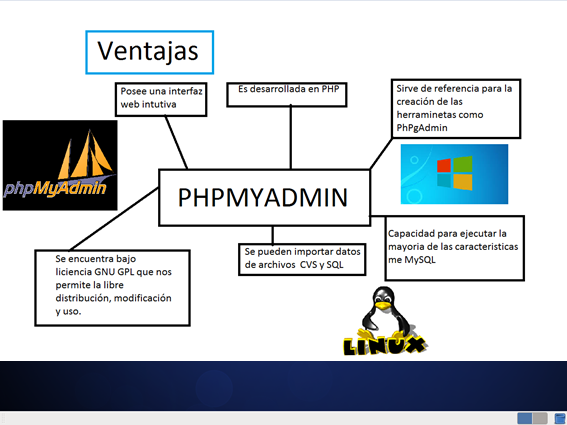
\includegraphics[width=12cm]{./Imagenes/a}
		\end{center}
\\\
\section{Características} 
\begin{itemize}
\\- Interfaz sobre web intuitiva.
\\- Proporciona herramientas de gestión de la base de datos:
\\- Edición, creación, modificación y eliminación de bases de datos, tablas, vistas, campos, relaciones e índices.
\\- Mantenimiento de usuarios y sus privilegios.
\\- Mantenimiento de procedimientos almacenados.
\\- Importación de datos desde CSV y SQL.
\\- Exportación a varios formatos: CSV,SQL, XML, PDF, SO/IEC 26300 - OpenDocument Text y Spreadsheet, Word, LATEX y otros.
\\- Administración de múltiples servidores.
\\- Creación del despliegue de la base de datos en un gráfico exportado a PDF.
\\- Creación de consultas complejas haciendo uso QBE (Query By Example).
\\

\end{itemize} 

\section{Requerimientos de Instalacion} 

        \begin{center}
		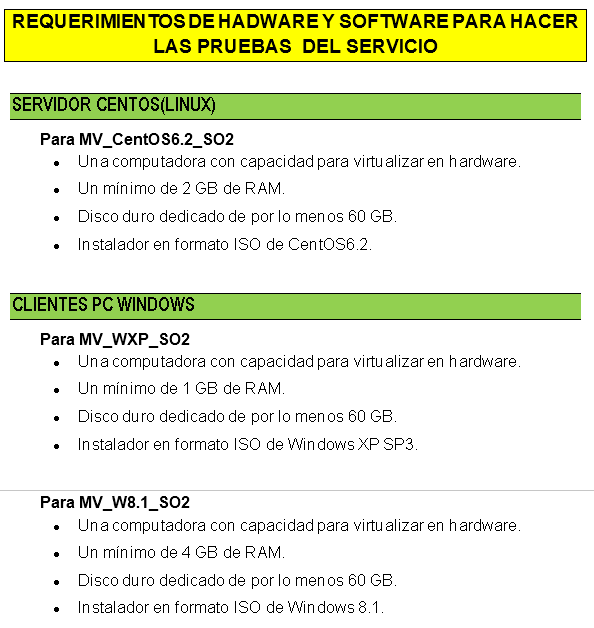
\includegraphics[width=13cm]{./Imagenes/b}
		\end{center}
		
		\begin{center}
		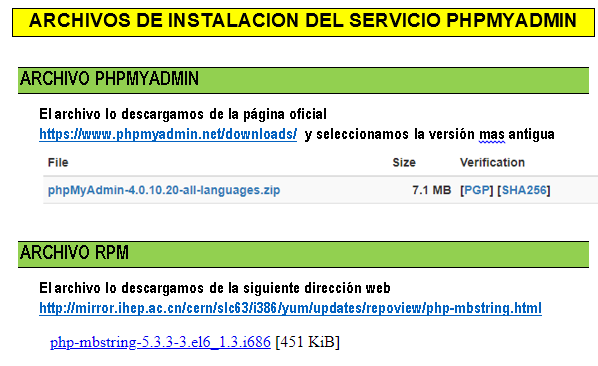
\includegraphics[width=13cm]{./Imagenes/c}
		\end{center}


\section{Instalación}

	\begin{center}
\item INSTALACIÓN DE SERVICIO PHPMYADMIN

    \end{center}
    
\end{itemize}

\begin{itemize}
		\begin{center}
		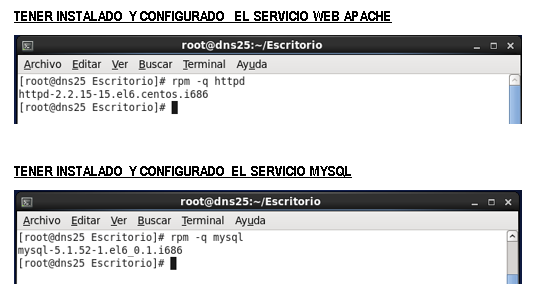
\includegraphics[width=15cm]{./Imagenes/d}
		\end{center}
\end{itemize}	
	\begin{itemize}
		\begin{center}
		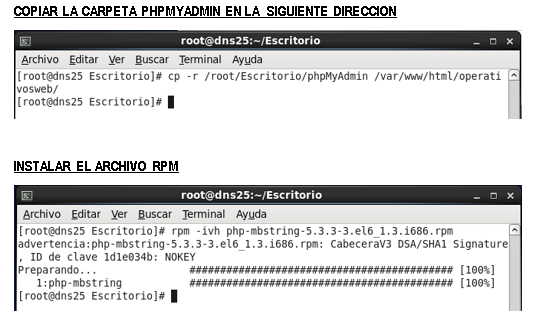
\includegraphics[width=15cm]{./Imagenes/e}
		\end{center}
\end{itemize}

	\begin{itemize}
		\begin{center}
		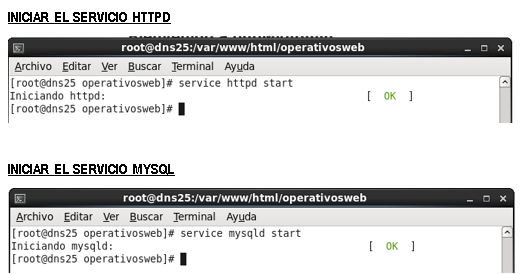
\includegraphics[width=15cm]{./Imagenes/f}
		\end{center}
\end{itemize}
\\\
\\\
\\\
\section{Configuración}
\begin{center}
\item CONFIGURACIÓN DE SERVICIO PHPMYADMIN
\end{center}
 
\end{itemize}

\begin{itemize}
		\begin{center}
		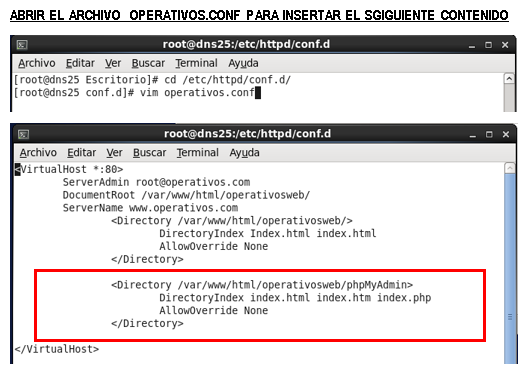
\includegraphics[width=15cm]{./Imagenes/g}
		\end{center}
\end{itemize}	
	\begin{itemize}
		\begin{center}
		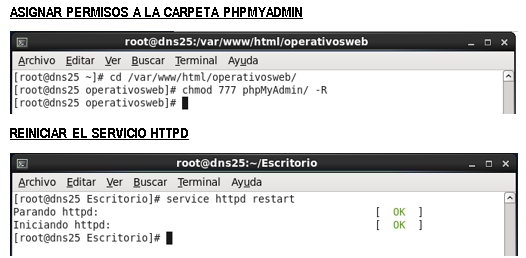
\includegraphics[width=15cm]{./Imagenes/h}
		\end{center}
\end{itemize}

\begin{itemize}
		\begin{center}
		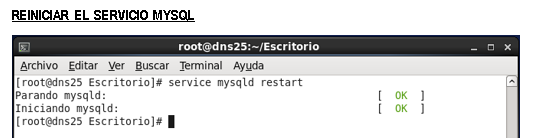
\includegraphics[width=15cm]{./Imagenes/i}
		\end{center}
\end{itemize}
		\\\
\section{Gestión y Administración}
\begin{center}
\item GESTIÓN Y ADMINISTRACIÓN DE PHPMYADMIN
\end{center}
 
\end{itemize}	
\begin{itemize}
		\begin{center}
		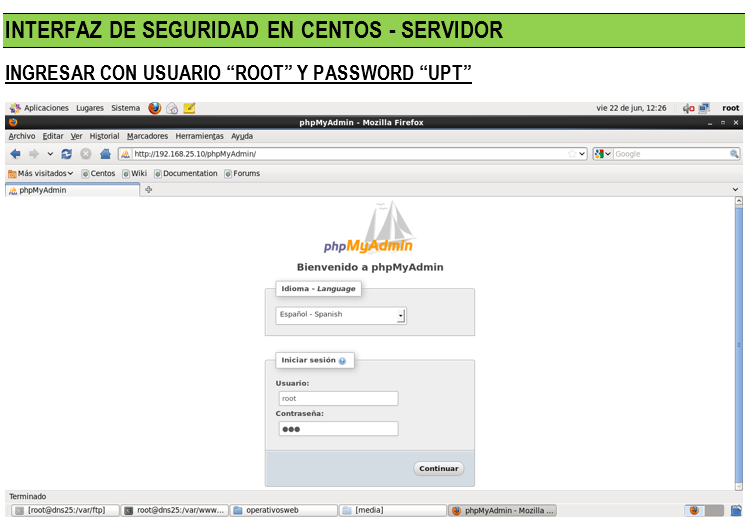
\includegraphics[width=15cm]{./Imagenes/j}
		\end{center}
\end{itemize}	

\begin{itemize}
		\begin{center}
		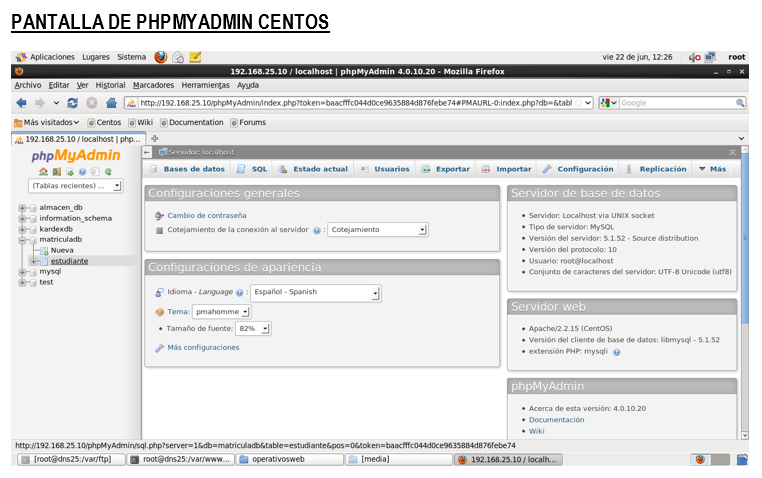
\includegraphics[width=15cm]{./Imagenes/k}
		\end{center}
\end{itemize}

\begin{itemize}
		\begin{center}
		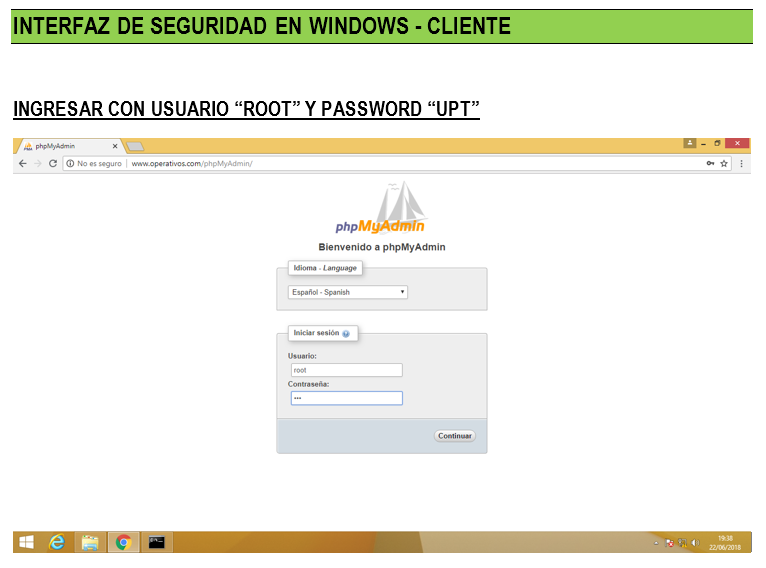
\includegraphics[width=15cm]{./Imagenes/l}
		\end{center}
\end{itemize}

\begin{itemize}
		\begin{center}
		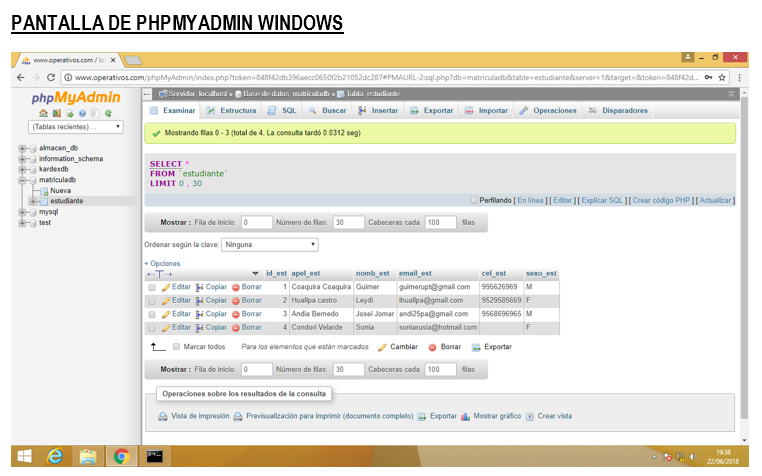
\includegraphics[width=15cm]{./Imagenes/m}
		\end{center}
\end{itemize}

\begin{itemize}
		\begin{center}
		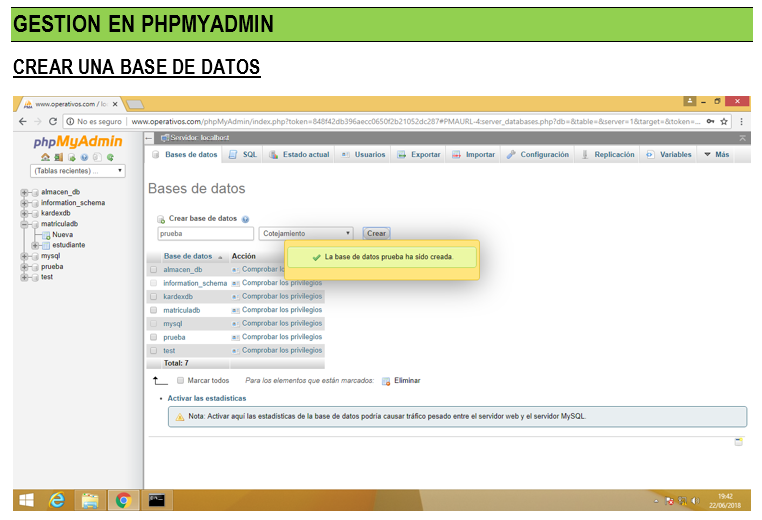
\includegraphics[width=15cm]{./Imagenes/n}
		\end{center}
\end{itemize}

\begin{itemize}
		\begin{center}
		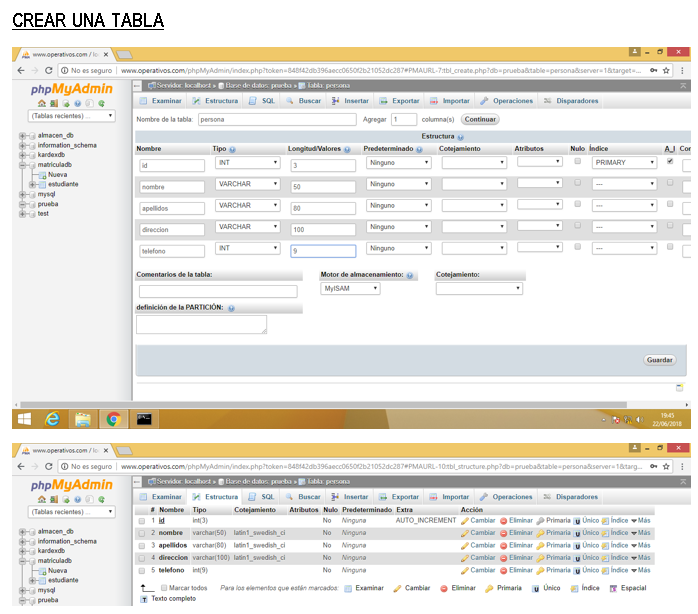
\includegraphics[width=15cm]{./Imagenes/nn}
		\end{center}
\end{itemize}

\begin{itemize}
		\begin{center}
		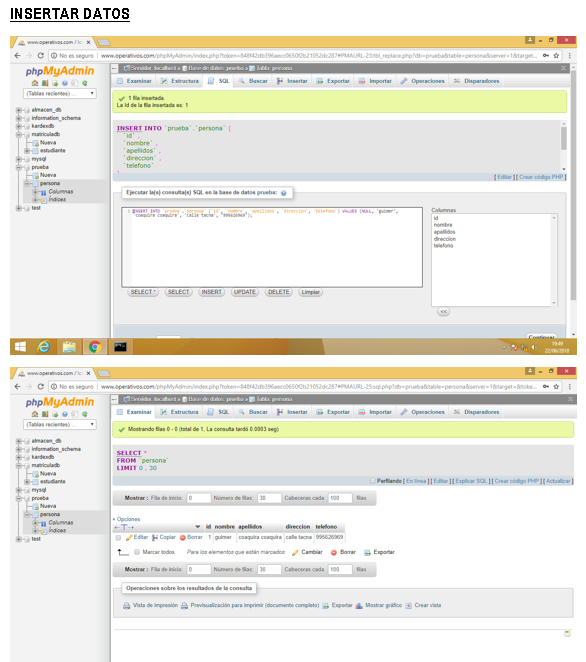
\includegraphics[width=15cm]{./Imagenes/o}
		\end{center}
\end{itemize}

\begin{itemize}
		\begin{center}
		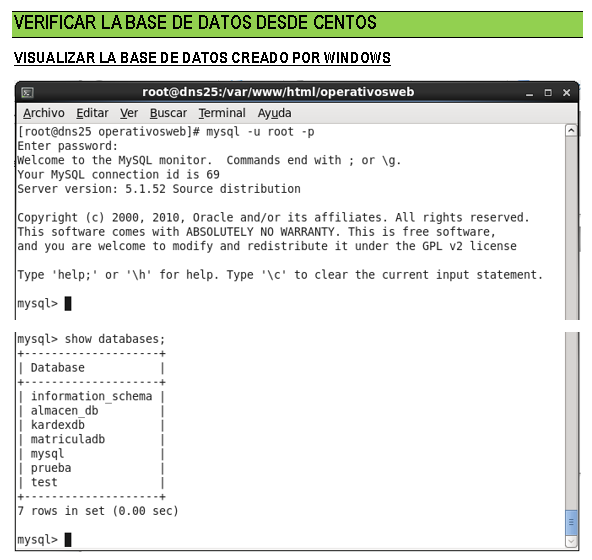
\includegraphics[width=15cm]{./Imagenes/p}
		\end{center}
\end{itemize}

\begin{itemize}
		\begin{center}
		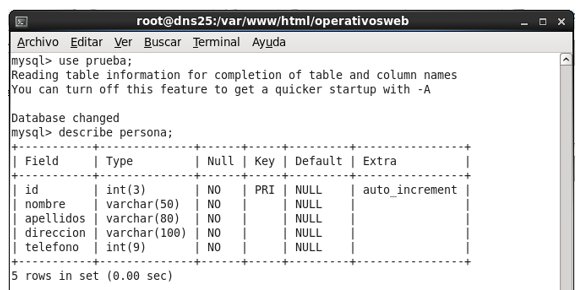
\includegraphics[width=15cm]{./Imagenes/q}
		\end{center}
\end{itemize}

\begin{itemize}
		\begin{center}
		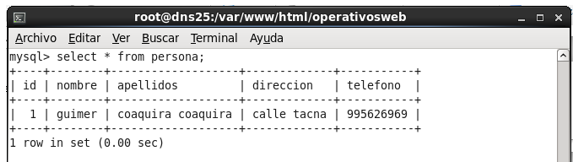
\includegraphics[width=15cm]{./Imagenes/r}
		\end{center}
\end{itemize}